%\VignetteIndexEntry{GPPFourier}

\documentclass[10pt,a4wide]{article}
\usepackage{graphicx}
\usepackage{lscape}
\usepackage{bm}
\usepackage{amsmath}
\usepackage{natbib}
\usepackage{Rd}

\newcommand{\Ox}{\mathrm{O_2}}

\author{Tom J.S. Cox}
\title{GPPFourier - An R package implementing the Fourier method to estimate Gross Primary Production from high frequency O2 data.}

\usepackage{Sweave}
\begin{document}
\Sconcordance{concordance:GPPFourier.tex:GPPFourier.Rnw:%
1 15 1 1 0 3 1 1 4 18 1 1 2 1 0 1 1 1 4 6 0 1 2 2 1 1 7 1 2 6 1 1 2 1 0 %
1 5 4 0 1 1 6 0 1 2 6 1 1 2 1 0 1 3 2 0 1 9 8 0 1 8 11 0 1 3 2 1 1 11 1 %
3 11 1}



\maketitle
\section{Introduction}

This package implements the Fourier method to estimate Gross Primary Production (GPP) from high frequency O2 data. This method estimates time averaged GPP as

\begin{eqnarray}
\overline{GPP(t)} \approx && 2 \omega_1 \frac{\sin \theta - \theta
\cos \theta}{\theta - \frac{1}{2}\sin 2\theta} A_{\Ox} \label{eq:final2}
\end{eqnarray}

where $A_{\Ox}$ represents the Fourier amplitude at the diurnal frequency of the oxygen time series; $\theta = \pi \mathrm{f_{DL}}$, with $\mathrm{f_{DL}}$ the relative fraction of daylight hours over a 24h period. $\omega_1$ denotes the diurnal frequency. For more details on the assumptions and performance of the method we refer to \citep{Cox2015b}.

The two core functions implementing the Fourier method are \texttt{GPPFourier()} and \texttt{GPPFourierPreprocess()}.\texttt{GPPFourier()} is the workhorse function of the package. It calculates GPP for a single time series of O2, regularly sampled at a fixed sampling rate. Before computing the Fourier amplitude at diel frequency, the time series is preconditioned with \texttt{GPPFourierPreprocess()}. This function allows for detrending and low pass filtering (simple moving average) the time series, and it confines the data set to an integer number of days. (it is called from within \texttt{GPPFourier()}).

Apart from the core functions, 2 higher level functions are provided to process a long data series in consecutive blocks of pre-defined length (\texttt{WindowGPPFourier()}) and to analyse multiple consecutive time series with a time gap in between, pasted together in a single data frame (\texttt{WindowGPPFourier.gts()}).

\section{Calculate GPP on a single oxygen time series}
Figure \ref{Fig1} shows a 10 day data set of oxygen observed at a fixed location in the Scheldt estuary (Kruibeke pontoon, N51.176 E4.326). The major visible oscilations are semi-diurnal due to the tides, that transport an oxygen gradient past the sensor. Nevertheless, there is a diel component in this time series, which is readily visible in a plot of the Fourier transform of the series (plotted with \texttt{plotF()}, Figure \ref{Fig1})

\begin{Schunk}
\begin{Sinput}
> par(mfrow=c(1,2))
> plot(DO,ylab="O2",type="l")
> plotF(detrend(DO$O2), 
+ 		dt=as.numeric(difftime(DO$time[2], DO$time[1], units="days")), 
+ 		xlim=c(0,3), 
+ 		type="b")
\end{Sinput}
\end{Schunk}

\begin{figure}[t]
\begin{center}
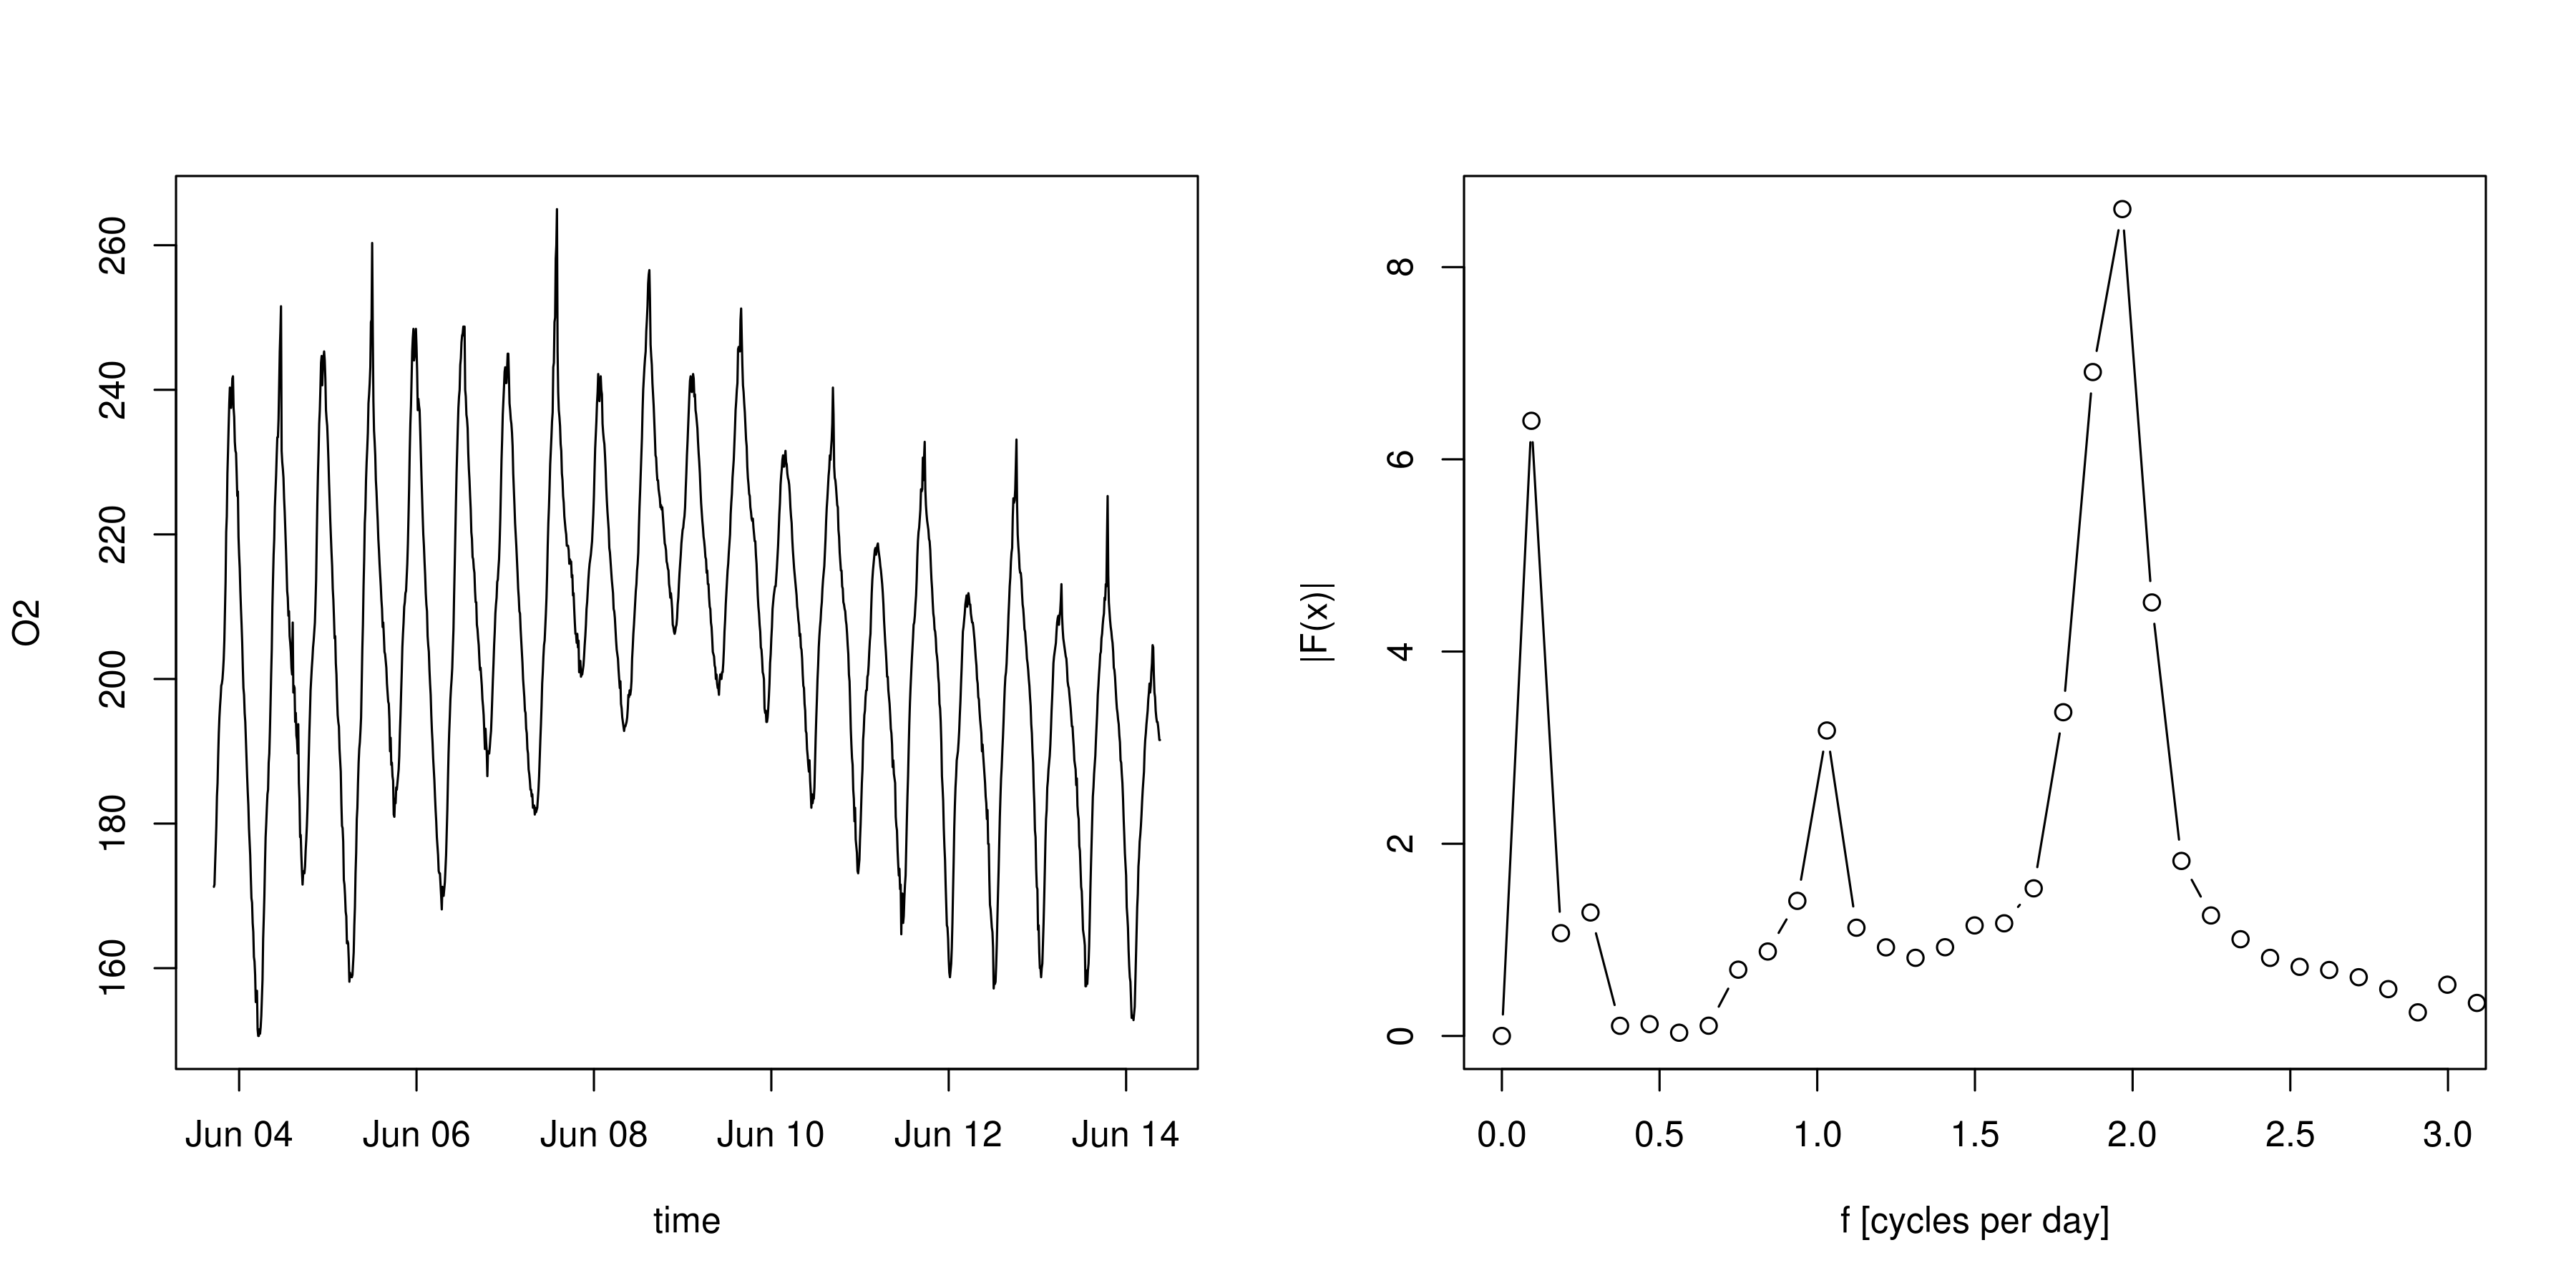
\includegraphics{GPPFourier-GPPFourierFig1}
\end{center}
\caption{Example O2 time series (left) and Fourier transform (right)} 
\label{Fig1}
\end{figure}

The function \texttt{GPFourier()} estimates average GPP over the period of this time series from the amplitude of the peak at the diel frequency. 

\begin{Schunk}
\begin{Sinput}
> dt <- difftime(DO$time[2], DO$time[1], units="days")
> GPP <- GPPFourier(DO$O2, 
+ 	dt=dt, 
+ 	Nfilt=1/as.numeric(dt, unit="days"), 
+ 	fDL=fDL(DO$time[1], phi=51.176, lambda=4.326)
+ )
> GPP # volume specific primary production, i.e. mu Mol O2/m3/d
\end{Sinput}
\begin{Soutput}
[1] 35.45083
\end{Soutput}
\end{Schunk}
This results in the volume specific gross primary production, with units given by the unit of the O2 concentration in the time series ($\mu$M) and the time unit of \texttt{dt} (days). Thus the GPP estimate from this $\Ox$ time series is 35.5 $\mu$M $\Ox$$m^{-3}d^{-1}$. The Fourier method assumes that the $\Ox$ time series represent the depth averaged $\Ox$ concentration, either because the system is considered vertically well mixed, or because the depth averaged concentrations is determined is explicitely observed, e.g. with multiple sensors. Thus, the surface specific productivity is obtained by simply multiplying by the depth of the system. The example data set is recorded at Kruibeke pontoon in the Scheldt estuary where the water depth is approximately 9.3m. Thus the surface specific productivity is estimated as 329.7 $\mu$M $\Ox$$m^{-2}d^{-1}$.

\section{Analysing multiple consecutive series}
Often, $\Ox$ sensor data consists of multiple consecutive series, each of them sampled at regular time intervals, interrupted by periods where there is no data available (due to sensor failure, maintenance,...). As an example, figure \ref{Fig2} presents the $\Ox$ data recorded in 2010 at a fixed location in the Scheldt estuary (Kruibeke pontoon, N51.176 E4.326). 

The function \texttt{WindowGPPFourier.gts()} analyses such interrupted $\Ox$ series with a single function call. It will split the time series at gaps that are larger that a specified number of data points (\texttt{gapMaxN}). On each individual series, GPP is caculated in consecutive time windows of prescribed length (\texttt{Width}). Missing values or gaps smaller than \texttt{gapMaxN} are automatically filled by linear interpolation. The result is shown in the bottom panel of figure \ref{Fig2}.

\begin{Schunk}
\begin{Sinput}
> par(mfrow=c(2,1))
> plot(O2_2010, 
+       pch=20,
+       xlim=as.POSIXct(c("2010-01-01", "2010-12-31")))
> GPPAll_4 <- WindowGPPFourier.gts(O2_2010, 
+                                   gapMaxN = 10, 
+                                   Width = 10, 
+                                   filtWidth=1*24, 
+                                   phi=51.176,
+                                   lambda=4.326, 
+                                   Detrend=TRUE, 
+                                   filter=TRUE, 
+                                   filtcorrect=FALSE)
> plot(GPPAll_4$time,
+       GPPAll_4$GPP*9.3/1.3, 
+       col="black", 
+       pch=19, 
+       type="b",
+       xlab="time", 
+       ylab="GPP", 
+       xlim=as.POSIXct(c("2010-01-01", "2010-12-31")))
> 
\end{Sinput}
\end{Schunk}

\begin{figure}[h]
\begin{center}
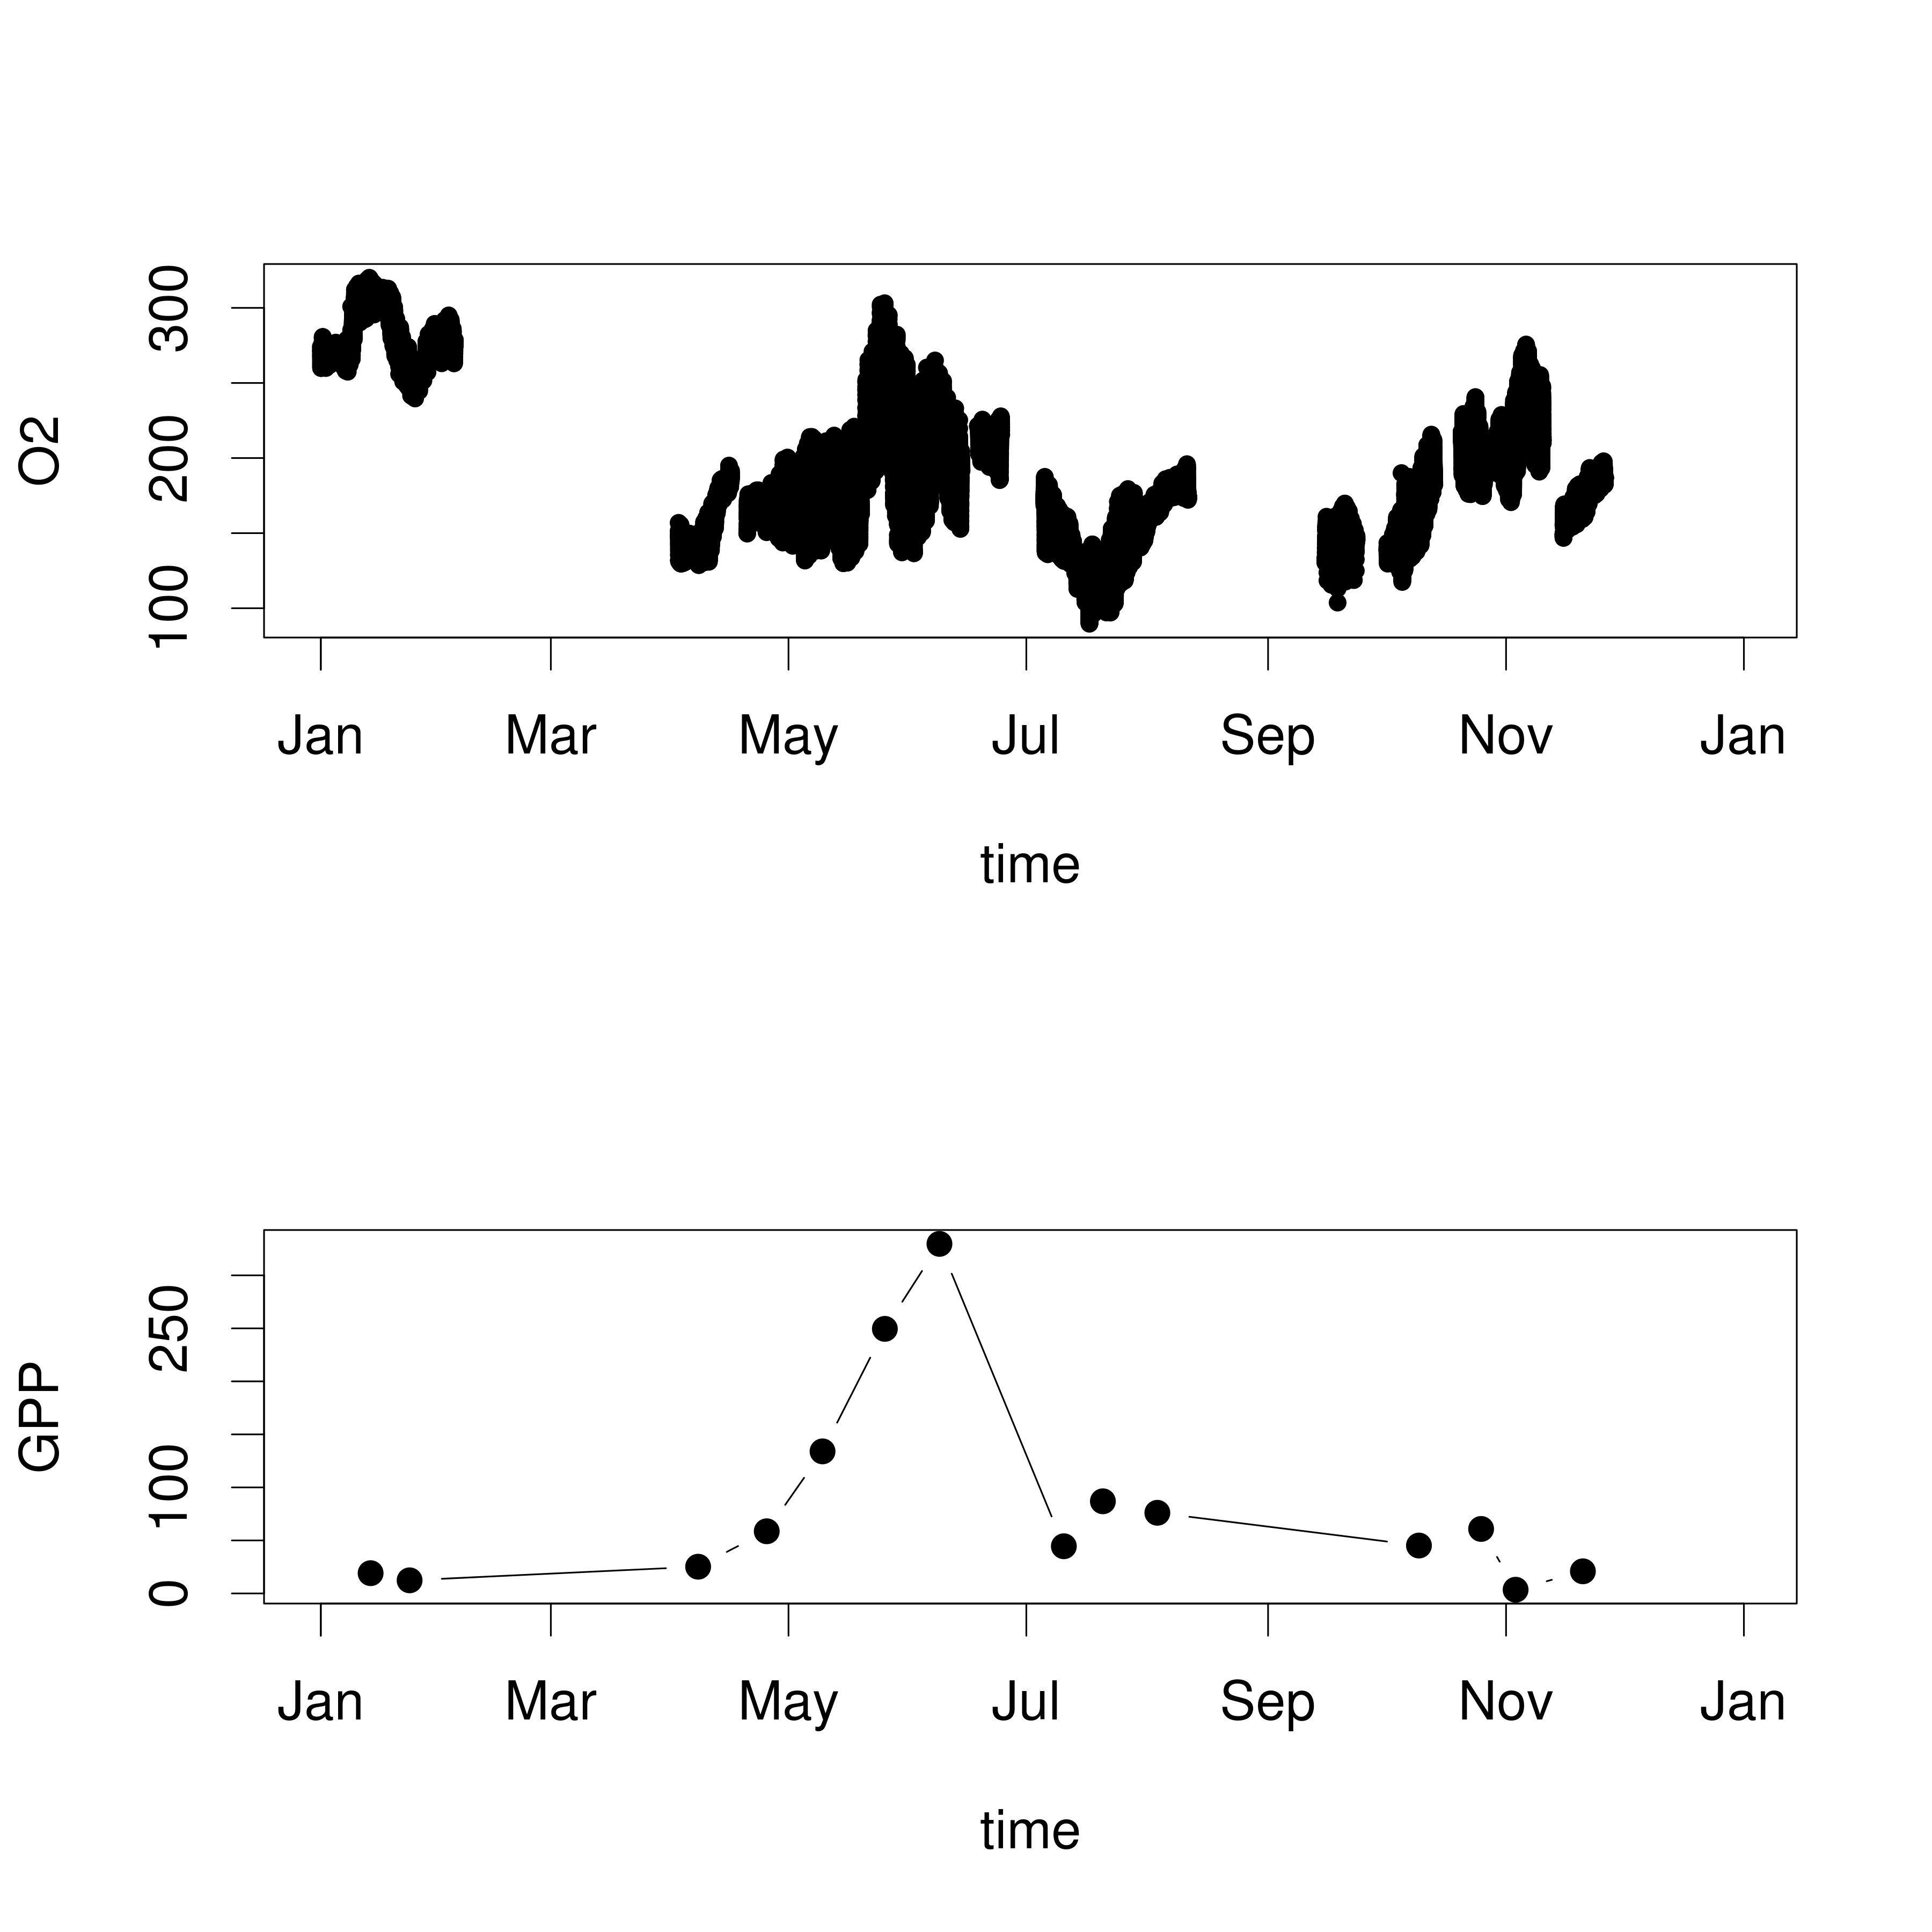
\includegraphics{GPPFourier-GPPFourierFig2}

\end{center}
\caption{Calculating GPP on multiple series at once} 
\label{Fig2}
\end{figure}



\bibliography{GPPFourier}
\bibliographystyle{apalike2}

\end{document}
